\chapter{Fejlesztői dokumentáció} % Developer guide
\label{ch:impl}

\section{Feladat specifikáció}
Az webalkalmazás célja egy működő webáruház bemutatása Angular keretrendszerben. Az alkalmazás két főrészre osztható kliensoldali (front-end) és egy szerveroldali (back-end) részre. A kliensoldal feladata a felhasználó által látott UI/UX megjelenítést biztosítsa. Amíg a szerveroldal felel a business logikáért, továbbá az adatok feldolgozásáért és hitelesítéséért.

\begin{figure}[H]
	\centering
	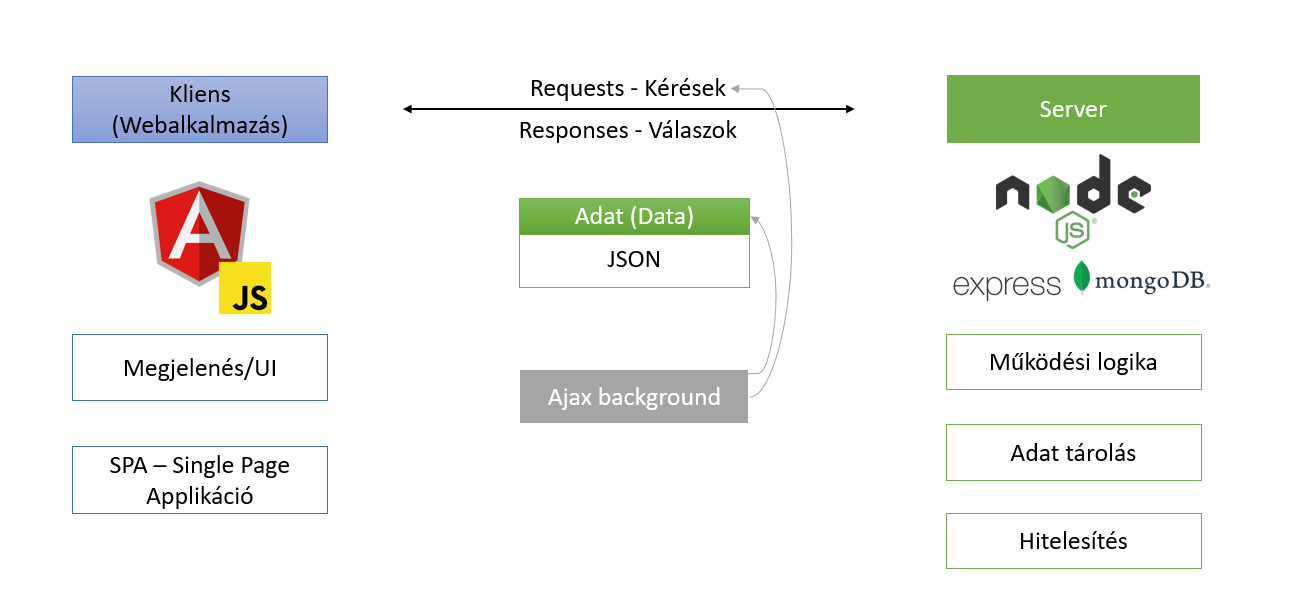
\includegraphics[width=1.0\textwidth,height=250px]{images/alkalmazas_bemutatasa.png}
	\caption{Az alkalmazás bemutatása}
	\label{fig.picture-1}
\end{figure}

A 3.1-es ábrán látható a két oldal kommunikációs kapcsolata. A front-end pontosabban mondva a kliensoldal Angular keretrendszerben TypeScript segítségével íródott. A front-end kommunikációja úgynevezett requestekkel más néven kérésekkel (json típusú adattovábbítással) történik amire a szerver oldal responsokkal egyszóval válaszokkal felel. A back-end NodeJS szoftverrendszer alapú, ami Express segítségével íródott. Az adatok tárolásáért a MongoDB nevezetű adatbázis felel.

\section{Webalkalmazás részletes bemutatása}

\subsection{Kliensoldalon használt technológiák bemutatása}

\subsection{Kliensoldal működése}

\subsection{Szerveroldalon használt technológiák bemutatása}

A következő fejezetben szeretném kifejteni a webáruház szerveroldali felépítését és az alkalmazásban használt technológiák működését. A 3.1-es ábrában felsorolt technológiákat részletesebben is szeretném bemutatni további grafikák segítségével.

\begin{figure}[H]
	\centering
	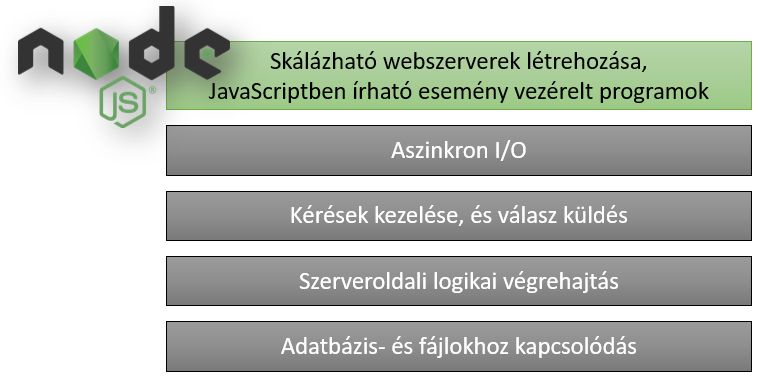
\includegraphics[width=1.0\textwidth,height=220px]{images/nodejs_bemutatasa.png}
	\caption{NodeJS bemutatása}
	\label{fig.picture-3}
\end{figure}

A webáruház back-end megírásánál 14.15.4-es verziójú Node.js szoftverrendszert használtam. A 3.2-es ábra látható a Node.js bemutatása, ami összefoglalja a szoftverrendszer fontosabb tulajdonságait. Az illusztráció első dobozában olvasható miszerint a Node.js skálázható webszerverek létrehozására alkalmas más szóval egy olyan rendszert tudunk létrehozni, ami több felhasználót képes egyidejűleg kiszolgálni. Továbbá JavaScript nyelv segítségével olyan programok írhatóak, amely a komponensek közötti esemény interakciókat tekinti alapul. Folytatólag a Node.js aszinkron tulajdonságával lehetővé teszi, hogy a kliensoldalról érkező kérések várakozási sorrendbe kerüljenek, ennek következtében a kliensoldal tovább folytathatja a feladatát. 

\begin{figure}[H]
	\centering
	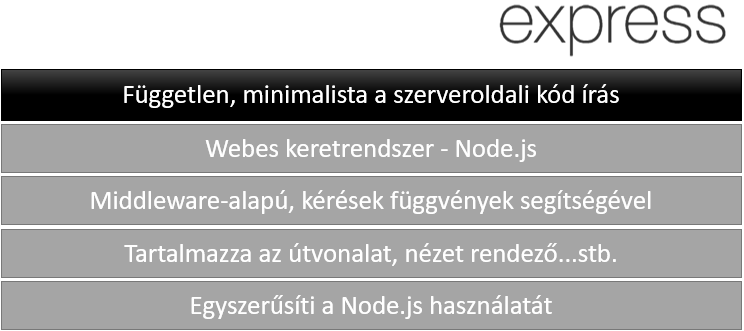
\includegraphics[width=0.8\textwidth,height=220px]{images/express_bemutatasa.png}
	\caption{Express bemutatása}
	\label{fig.picture-4}
\end{figure}

A szerveroldal áttekinthetőbb és olvashatóbb kódírás érdekében a webáruház fejlesztése során az Express 4.17.1-es verzióját használtam. Az Express egy webes keretrendszer a Node.js nehézség nélküli használatához. A 3.3-as ábrán látható az Express attribútumainak ismertetése. Az illusztráción felvetettem, hogy az Express egy Middleware-típusú rendszer következésképpen lehetővé teszi a mongoDB adatbázis szoftverhez való zavartalan kapcsolódást a Mongoose 6.0.12 verziójával kiegészítve, ami egy JavaScript-ben írt objektum-orientált programozási könyvtár.

\begin{figure}[H]
	\centering
	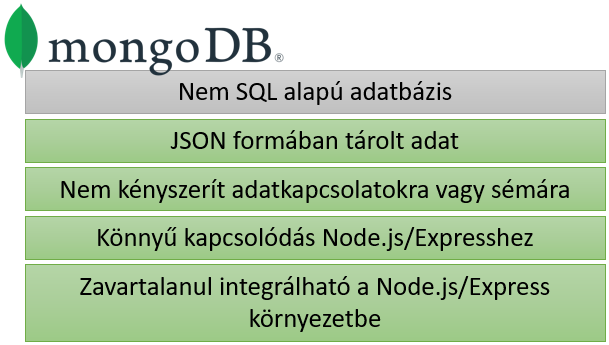
\includegraphics[width=0.8\textwidth,height=220px]{images/mongodb_bemutatasa.png}
	\caption{mongoDB bemutatása}
	\label{fig.picture-5}
\end{figure}

\begin{description}
	\item[A mongoDB]egy nyílt forráskódú, NoSQL adatbázisszerverek közé sorolt szoftver. A NoSQL magyarán Nem SQL típusú adatbázisrendszert jelent. Jellemzően nem rekordokat és táblázatokat tárolnak, hanem független dokumentumokat és gyűjteményeket archiválnak. Személyes véleményem szerint a 3.4-es illusztrációval alátámasztva egyik legfőbb pozitív tulajdonságának éreztem a alkalmazás írása során, hogy az adatok JSON formátumban képes tárolni. Következésképpen a request és response folyamatok egyszerűsített és gyors működését képes biztosítani, mindeközben lehetővé teszi a kliensoldalon megjelenítendő információk könnyebb feldolgozását. 
\end{description}
 
A következő grafikai ábrán szándékozom röviden bemutatni és összehasonlítani a Nem SQL és az SQL alapú adatbázisok jellegzetes tulajdonságaik szerint.

\begin{figure}[H]
	\centering
	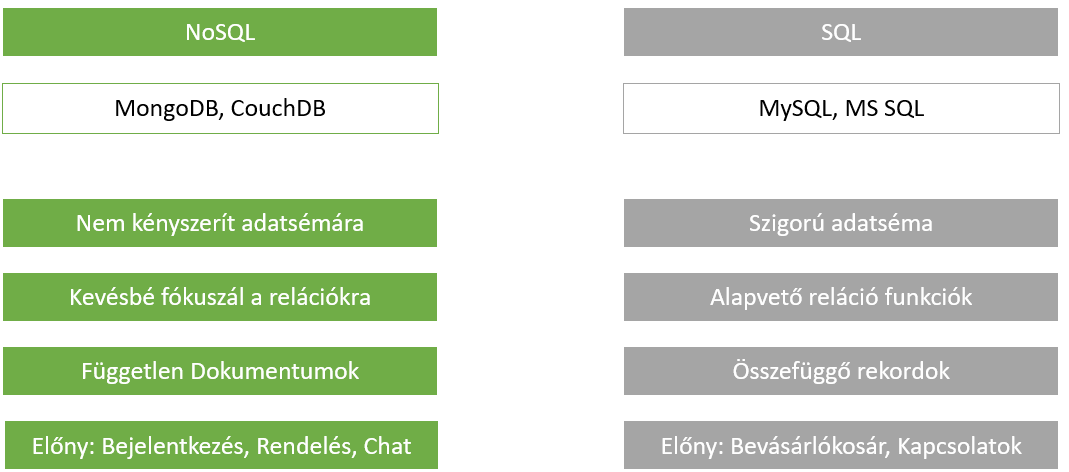
\includegraphics[width=1.0\textwidth,height=220px]{images/nosql_bemutatasa.png}
	\caption{NoSQL vs SQL adatbázisok összehasonlítása}
	\label{fig.picture-6}
\end{figure}

A NoSQL adatbázisszerverek jellemzői kulcsfontosságú szempontokat szolgált a webáruház megírásához.

\subsection{Szerveroldal működése}

Ebben a fejezetben szeretném részletesen prezentálni a webalkalmazásom szerveroldali működését példának okáért milyen request és response hívások találhatóak a kódban, hogyan létesít kapcsolatot a webalkalmazás az adatbázissal...stb.

\begin{description}
	\item[A webáruház megírása során RESTful API-t] (feloldva: Representational State Transfer Application programming interface) magyarán reprezentáción alapuló állapotátvitel nevezetű architekturális módszert használtam. Az API-k segítségével a felhasználó számára elérhető az alkalmazással történő számos interakció.
	
	\item[Az alábbi illusztráción] szeretném bemutatni az általam használt REST API hívásokat, ennek okán a 3.6-os ábrán láthatók a programban megírt végpontok.
\end{description}

\begin{figure}[H]
	\centering
	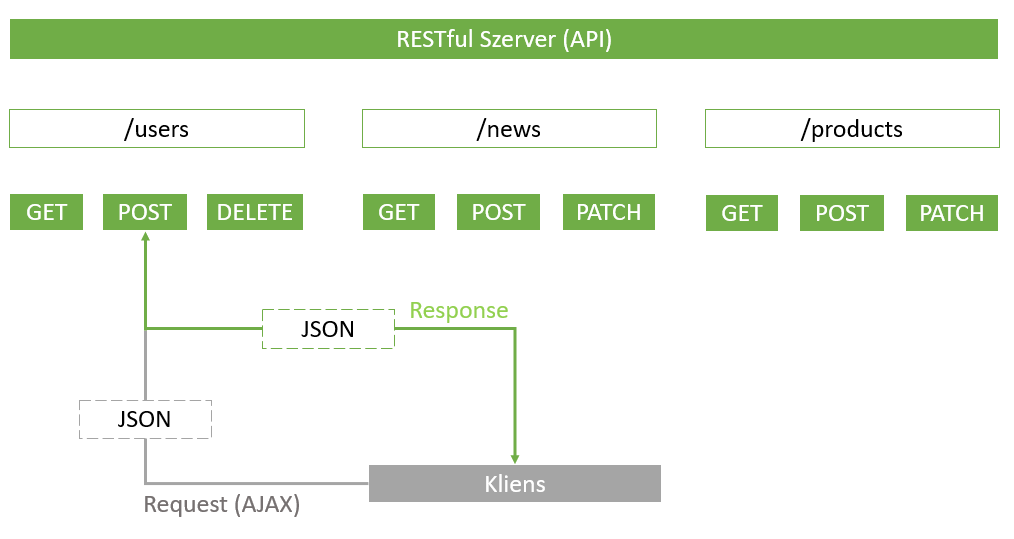
\includegraphics[width=1.0\textwidth,height=220px]{images/restapi_bemutatasa.png}
	\caption{Adatkezelés}
	\label{fig.picture-8}
\end{figure}

 A grafikán megfigyelhető hat különböző végpont ami a auth, hírek, termékek, termékcsoportok, üzenetek és rendeléseket fejezi ki. Az illusztrációt figyelemmel kísérve identifikálható, hogy nem minden végpont rendelkezik ugyan azokkal a kérésekkel. Szemléltetésképp vegyük figyelembe a hírekhez vonatkozó responsokat amik a GET, POST, PATCH és DELETE függvények ezzel szemben a auth-hoz kizárólag POST függvény tartozik.

\begin{description}
	\item[A REST API]-t megismerve és ezt az információt felhasználva kívánom szemléltetni és alább bemutatni a következő grafikán miképpen éri el a felhasználó által kezdeményezett kérése az adatbázist.
\end{description}

\begin{figure}[H]
	\centering
	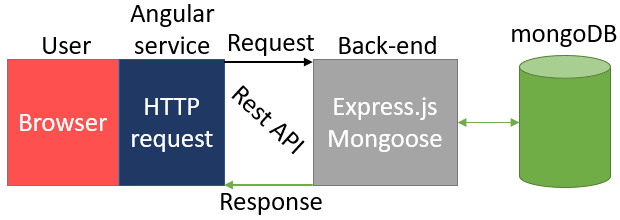
\includegraphics[width=1.0\textwidth,height=220px]{images/kapcsolat_szerver_bemutatas.png}
	\caption{Kapcsolat a szerverrel}
	\label{fig.picture-7}
\end{figure}

A fenti 3.7-es ábrán kifejezetten látható milyen sorrendben jut el az adatbázishoz a felhasználó által indított kérés és miképpen tér vissza hozzá.

\begin{description}
	\item[Az alkalmazás megírása során] akaratlagosan egy olyan webáruház létrehozása volt a végcélom, ami időszerű adatok kezelését tudja biztosítani. Következésképpen egy olyan felület megvalósítása gyakorlatban, amely nem igényel programozón keresztüli beavatkozást. Ennek okán a szakdolgozat tartalmaz egy adminisztrációs oldal, amely biztosítja az alkalmazásban dinamikusan megjelenő adatok aktualitását, továbbá a leadott rendelések vásárlók által elküldött üzenetek megjelenítésére is szolgál. Kifejezetten ennek a blokk védelmében került bele külön hitelesítési felület.
\end{description}
 
 Az alább található 3.8-as grafikán ez az engedélyezési folyamat ismertetése látható.
 
\begin{figure}[H]
	\centering
	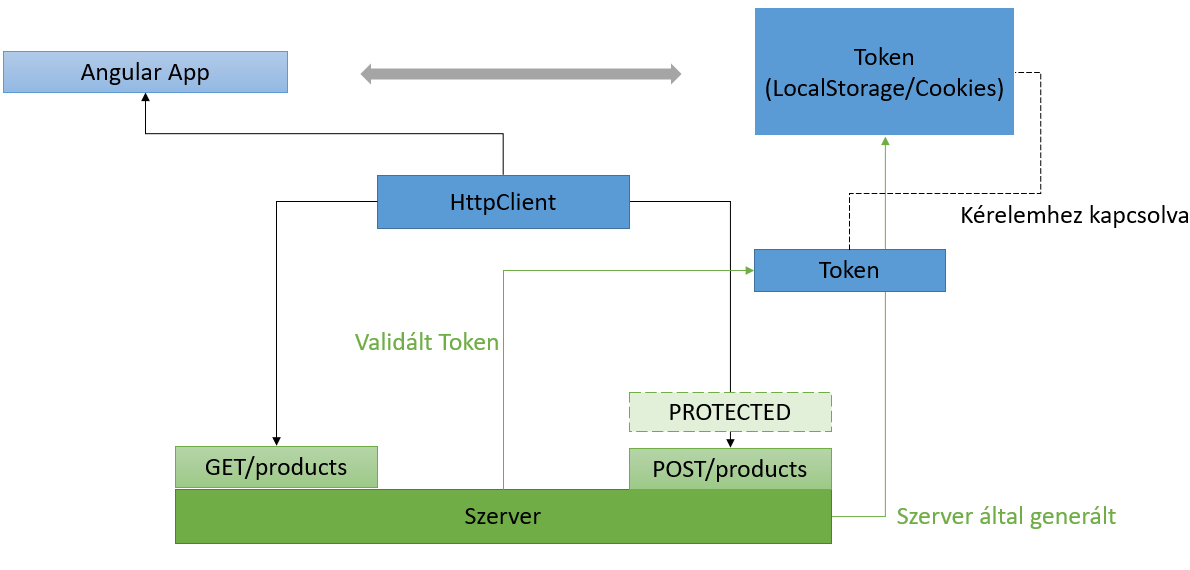
\includegraphics[width=1.0\textwidth,height=220px]{images/hitelesites_bemutatasa.png}
	\caption{Hitelesítés}
	\label{fig.picture-9}
\end{figure}

Az illusztráción ábrázolt hitelesítési folyamat a következőképpen történik. Az alkalmazás front-end-ről érkező GET/products kérésre engedélyezés nélkül kap választ a szervertől, mivel a webáruházban bejelentkezés hiányában is hozzáférhetővé kell tenni ezt az információt. Ezzel szemben a POST/products kérés nem következhet be hitelesítés nélkül. Tehát bejelentkezés során a szerver generál és LocalStorage-ba elment egy úgynevezett tokent, amit az új termék hozzáadás kérésnél ellenőriz. Mindent összevetve a POST kérés védve van a szükséges tokennel nem rendelkezőktől.

\section{Tételek, definíciók, megjegyzések} % Theorem-like items

\begin{definition}
Mauris tristique sollicitudin ultrices. Etiam tristique quam sit amet metus dictum imperdiet. Nunc id lorem sed nisl pulvinar aliquet vitae quis arcu. Morbi iaculis eleifend porttitor.
\end{definition}

Maecenas rutrum eros sem, pharetra interdum nulla porttitor sit amet. In vitae viverra ante. Maecenas sit amet placerat orci, sed tincidunt velit. Vivamus mattis, enim vel suscipit elementum, quam odio venenatis elit, et mollis nulla nunc a risus. Praesent purus magna, tristique sed lacus sit amet, convallis malesuada magna. Phasellus faucibus varius purus, nec tristique enim porta vitae.

\begin{theorem}
Nulla finibus ante vel arcu tincidunt, ut consectetur ligula finibus. Mauris mollis lectus sed ipsum bibendum, ac ultrices erat dictum. Suspendisse faucibus euismod lacinia. Etiam vel odio ante.
\end{theorem}
\begin{proof}
Etiam pulvinar nibh quis massa auctor congue. Pellentesque quis odio vitae sapien molestie vestibulum sit amet et quam. Pellentesque vel dui eget enim hendrerit finibus at sit amet libero. Quisque sollicitudin ultrices enim, nec porta magna imperdiet vitae. Cras condimentum nunc dui.
\end{proof}

Donec dapibus sodales ante, at scelerisque nunc laoreet sit amet. Mauris porttitor tincidunt neque, vel ullamcorper neque pulvinar et. Integer eu lorem euismod, faucibus lectus sed, accumsan felis. 

\begin{remark}
Nunc ornare mi at augue vulputate, eu venenatis magna mollis. Nunc sed posuere dui, et varius nulla. Sed mollis nibh augue, eget scelerisque eros ornare nec. Praesent porta, metus eget eleifend consequat, eros ligula eleifend ex, a pellentesque mi est vitae urna. Vivamus turpis nunc, iaculis non leo eget, mattis vulputate tellus.
\end{remark}

Fusce in aliquet neque, in pretium sem. Donec tincidunt tellus id lectus pretium fringilla. Nunc faucibus, erat pretium tempus tempor, tortor mi fringilla neque, ac congue ex dui vitae mauris. Donec pretium et quam a cursus.

\begin{note}
Aliquam vehicula luctus mi a pretium. Nulla quam neque, maximus nec velit in, aliquam mollis tortor. Aliquam erat volutpat. Curabitur vitae laoreet turpis. Integer id diam ligula.
\end{note}

Ut sollicitudin tempus urna et mollis. Aliquam et aliquam turpis, sed fermentum mauris. Nulla eget ex diam. Donec eget tellus pharetra, semper neque eget, rutrum diam.


\section{Forráskódok} % Source code samples

\subsection{Kliensoldali forráskódok}
Nulla sodales purus id mi consequat, eu venenatis odio pharetra. Cras a arcu quam. Suspendisse augue risus, pulvinar a turpis et, commodo aliquet turpis. Nulla aliquam scelerisque mi eget pharetra. Mauris sed posuere elit, ac lobortis metus. Proin lacinia sit amet diam sed auctor.

\subsection{Szerveroldali forráskódok}
Alább található forráskódok a 3.2.4-es fejezetben már meg említett Express.js-ben írt egy-egy példa request végpontokat tartalmazza.

POST/news~\ref{src:post} and \ref{src:csharp}:

\lstset{caption={POST/news végpont}, label=src:post}
%\begin{lstlisting}[language=javascript]
%exports.postNews = (req, res, next) => {
%	const url = req.protocol + "://" + req.get("host");
%	const news = new News({
%		title: req.body.title,
%		description: req.body.description,
%		imagePath: url + "/images/news/" + req.file.filename,
%		startDate: req.body.startDate,
%		endDate: req.body.endDate,
%	});
%	news.save().then(result => {
%		res.status(201).json({
%			message: "News added successfully",
%			news: {
%				...result,
%				id: result._id
%			}
%		});
%	});
%}
%\end{lstlisting}

\lstset{caption={Hello World in C\#}, label=src:csharp}
\begin{lstlisting}[language={[Sharp]C}]
using System;
namespace HelloWorld
{
	class Hello 
	{
		static void Main() 
		{
			Console.WriteLine("Hello World!");
			
			Console.WriteLine("Press any key to exit.");
			Console.ReadKey();
		}
	}
}
\end{lstlisting}

\subsection{Algoritmusok} % Algorithms

A general Interval Branch and Bound algorithm is shown in Algorithm~\ref{alg:ibb}. One of the following selection rules is applied in Step \ref{step:selrule}.\\
Példa forrása: \href{https://www.inf.u-szeged.hu/actacybernetica/}{Acta Cybernetica (ez egy link)}.

\begin{algorithm}[H]
\caption{A general interval B\&B algorithm} 
\label{alg:ibb} 
\textbf{\underline{Funct}} IBB($S,f$)
\begin{algorithmic}[1] % sorszámok megjelenítése minden n. sor előtt, most n = 1
\State Set the working list ${\cal L}_W$ := $\{S\}$ and the final list ${\cal L}_Q$ := $\{\}$     
\While{( ${\cal L}_W \neq \emptyset$ )} \label{alg:igoend}
	\State  Select an interval $X$ from ${\cal L}_W$ \label{step:selrule}\Comment{Selection rule}  
	\State Compute $lbf(X)$ \Comment{Bounding rule}		  
	\If{$X$ cannot be eliminated} \Comment{Elimination rule}
		\State Divide $X$ into $X^j,\ j=1,\dots, p$, subintervals   \Comment{Division rule}
		\For{$j=1,\ldots,p$}
			\If{$X^j$ satisfies the termination criterion} \Comment{Termination rule}
				\State Store $X^j$ in ${\cal L}_W$ 
			\Else
				\State Store $X^j$ in ${\cal L}_W$ 
			\EndIf
		\EndFor  
	\EndIf
\EndWhile
\State \textbf{return} ${\cal L}_Q$
\end{algorithmic}
\end{algorithm}
